\section{Experiments}
\label{sec:results}
To demonstrate our superiority over existing methods on biomedical segmentation, we present the results on two challenging biomedical problems, including synaptic vesicle segmentation and gland segmentation.
%To demonstrate the easy extension and generic applicability of our framework, we modified our DSAN to scene text segmentation task.

\subsection{Synaptic vesicle segmentation}
\noindent\textbf{Dataset}
Synaptic vesicle is a good example to evaluate our method, as most of vesicle shape are approximatively ellipse shape.
The images were acquired by cryo-electron tomography, which suffers from high noisy by deficient imaging technique.
The synaptic samples are obtained by frozen-hydrated culture neurons.
The plausible vesicles in image are densely arranged and easily confused with other membrane in presynaptic cells, therefore it is hard to obtain clear contour for such dense and small objects.
Our original dataset is composed of $120$ images with annotations provided by biologists.
The height and width of each image are respectively $1019$ and $1053$, averagely containing $200$ vesicle objects.
Since the average length of a vesicle is about $30$ pixels, we crop a $321\times 321$ region following \cite{Chen2014a} from the original image as the input to network so that each cropped image contains about $25$ objects.
We uniformly crop $25$ patches in each original image with overlap, and use a data augmentation strategy, including translation, rotation and image flipping.
Finally the dataset consists of $8787$ images is used for training and evaluation.
Especially, a six-fold cross validation is applied in our experiments.

\noindent\textbf{Implementation details.}
We train our network on the open-source deep learning library Caffe~\cite{Jia2014}.
%All the experiments are implemented on a workstation with TitanX GPU cards.
The model of DSAN is well trained by a two-step process.
In the first stage, we independently train the segmentation branch as a general segmentation task following \cite{Chen2014a}.
The base learning rate was set as $10^{-3}$ and a `step' policy is adopted by decreasing the learning rate by a fact of $10$ every $2000$ iterations.
And mini-batch size was set to $30$ for one iteration with the max iteration number $20000$.
In the second stage, the multi-task FCN as well as $M$ sequential SMP layers is jointly fine-tuned based on the model from the first stage.
The learning rate drops to $10^{-8}$, and the iteration number in the second stage is set as $8000$.
The balancing weight $\lambda$ in Eq.~\ref{EqLoss} and $\alpha$ in Eq.~\ref{dG} are experimentally set to be $10^{-4}$ and $10^{-3}$.
Especially, $M$, $k_s$, $\tau_1$ and $\tau_2$ will be jointly explored in latter experiment.

\noindent\textbf{Evaluation setup.}
%
The evaluation criteria in our experiments includes a score $F_1$ \cite{Chen2016a} to evaluate performance of object detection and a pixel intersection-overunion (IOU) averaged across different classes \cite{Chen2014a} to evaluate  the segmentation accuracy .
Especially, the evaluation criteria in gland segmentation task uses the object-level Dice index (Dice) metric defined in \cite{Chen2016a} to evaluate the object-level segmentation performance.
%The $F_1$ score considers the performance of object detection, while IOU consider the segmentation performance, respectively.
\begin{figure}
    \begin{center}
        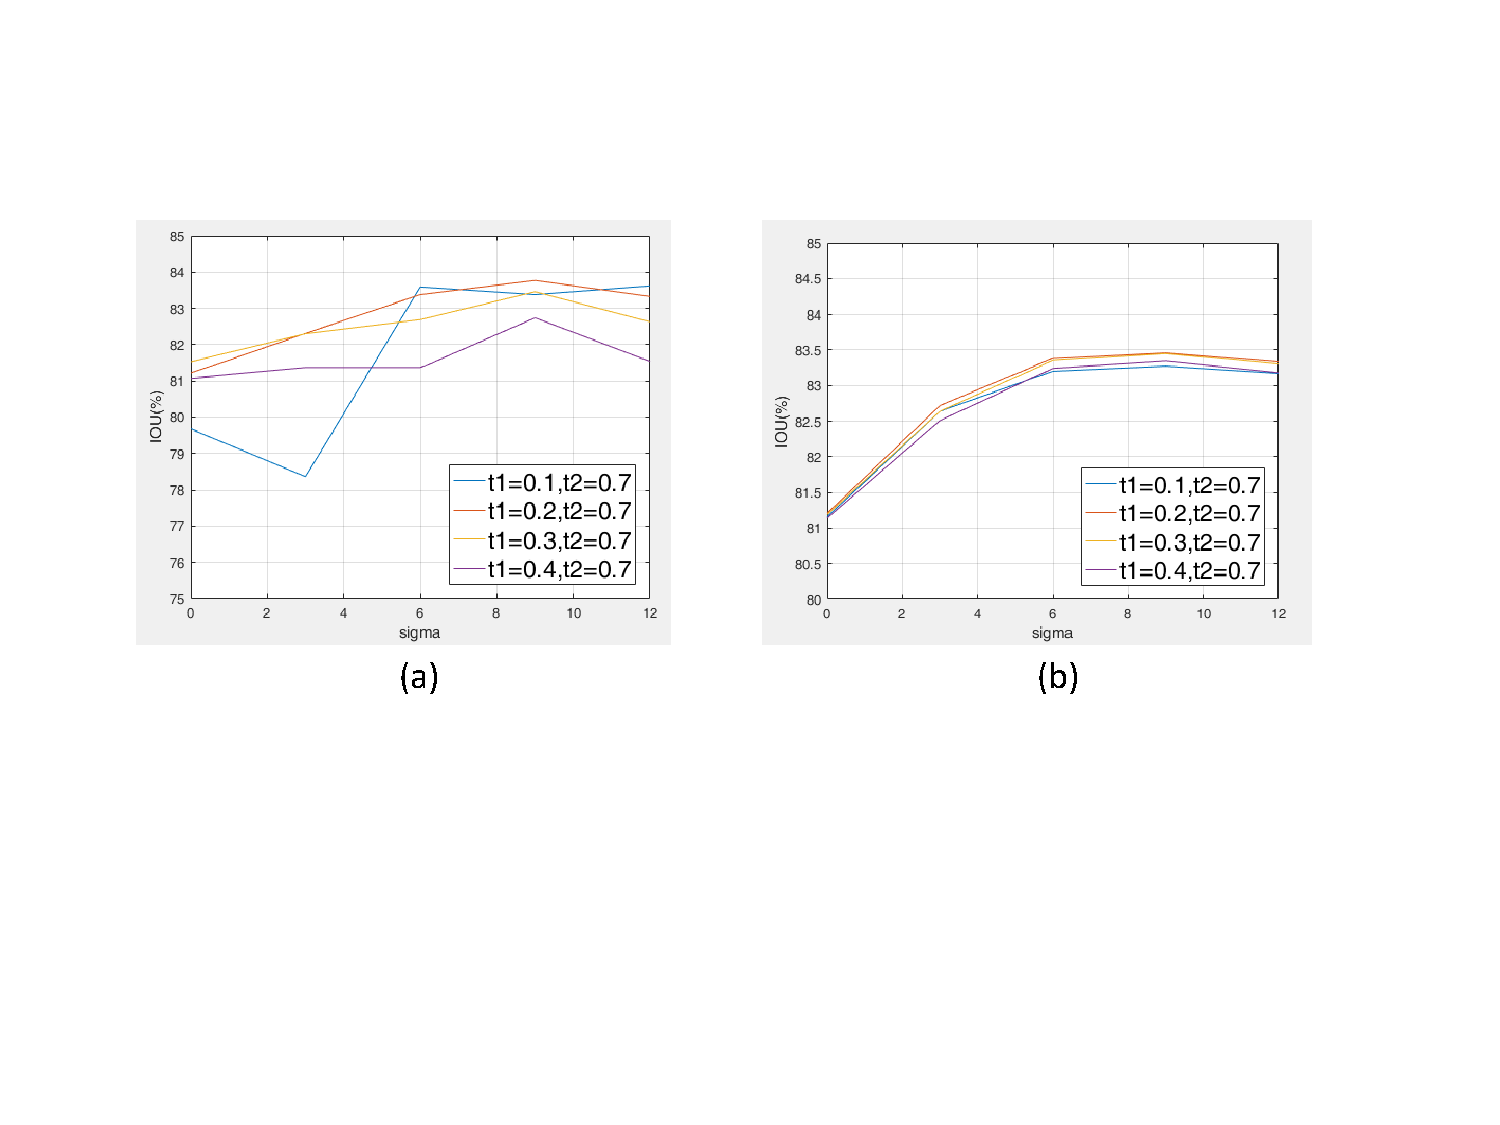
\includegraphics[width=3.3in]{figures/FigVar.pdf}
   %\includegraphics[width=0.8\linewidth]{egfigure.eps}
    \end{center}
    \caption{Effect of varying $\varepsilon$ for vesicle segmentation: (a)Fix $\tau_2$ and vary both $\tau_1$ and $\varepsilon$. (b) Fix $\tau_1$ and vary both $\tau_2$ and $\varepsilon$.}
    \label{FigVar}
\end{figure}

\begin{table}
\begin{center}
\begin{tabular}{l|ccccc}
\hline
$\tau_1,\tau_2$ & 0.5,0.5 & 0.4,0.6&0.3,0.7&0.2,0.8&0.1,0.9\\
\hline
$L_{aux}$&0.089&0.089&0.085&0.078&$\mathbf{0.070}$\\
\hline
IOU(\%)&79.66& 81.37&82.60&$\mathbf{83.62}$&83.30\\
\hline
F1(\%)&68.67&72.08&75.29&77.41&$\mathbf{78.88}$\\
\hline
\end{tabular}
\end{center}
\caption{Effects of using different $[\tau_1,\tau_2]$.
        $L_{aux}$ is the error of predicted shape parameters.
        $\tau_1=\tau_2$ means no split max pooling used for DSAN.}
\label{tab:var}
\end{table}

\noindent\textbf{Exploring the effect of $\{M, k_s, \tau_1, \tau_2\}$ to final segmentation.}
In this experiment, the effects of different $M$, $k_s$, $\tau_1$, $\tau_2$ on the segmentation performance are jointly investigated.
In order to reduce the hyper-parameters, we use $\varepsilon=\frac{(M-1)k_s}{2}$ to represent the effect of both $M$ and $k_s$ , because they have similar effects on SMP of changing the spreading range of a local maximum value.
Especially, $\varepsilon=0$ means no split max pooling applying to the network.
First, we fix $\tau_2=0.7$ and vary $\tau_1$ to observe its influence of different $\varepsilon$ in DSAN model as shown in Figure~\ref{FigVar}~(a).
Then, $\tau_1$ is fixed and $\tau_2$, $\varepsilon$ are varied in Figure~\ref{FigVar}~(b).
Observed from Figure~\ref{FigVar}, it is properly to employ $\varepsilon=9$ for vesicle segmentation to obtain most of the gains for different $\tau1$ and $\tau2$.
In practice, we set $k_s=9$ and $K=3$ to satisfy the condition of $\varepsilon=9$ as well as for efficiently implementing DSAN.
For $\tau_1$ in Figure~\ref{FigVar} (a), we find that $\tau_1=0.2$ is the best setting when $\varepsilon=9$.
And fixing $\tau_1=0.2$, $0.9$ is found to be optimal for $\tau_2$ according to Figure~\ref{FigVar} (b).
After searching the optimal $\tau_1$ and $\tau_2$, Table~\ref{tab:time} evaluates the effects of different $M$ and $k_s$ by fixing $\frac{(M-1)k_s}{2}=9$.
From Table~\ref{tab:time}, the effects of $M$ and $k_s$ on inference times are small, thus we use $M=3$ and $k_s=3$ in rest experiments. 
Finally, we find that the thresholds setting of $[0.2, 0.9]$ in Eq.~\ref{fusion} give the best performance on segmenting synaptical vesicles.

Furthermore, table~\ref{tab:var} shows the results of several interval of $[\tau_1,\tau_2]$, where the $L_{aux}$ indicates the second loss term in Eq.~\ref{EqLoss}.
From the table, it can be found that the loss of predicted shape parameters becomes small after using split max pooling layers, confirming our hypothesis illustrated in Sec.~\ref{sec:split-max-pooling}.
And from the IOU score and F1 score, we find that too strong shape constraint on segmented object by a larger interval of $[\tau_1,\tau_2]$ is harmful to the IOU score but beneficial to the F1 score, which has been illustrated in Sec.~\ref{sec:fusion}.
\begin{figure*}
    \begin{center}
        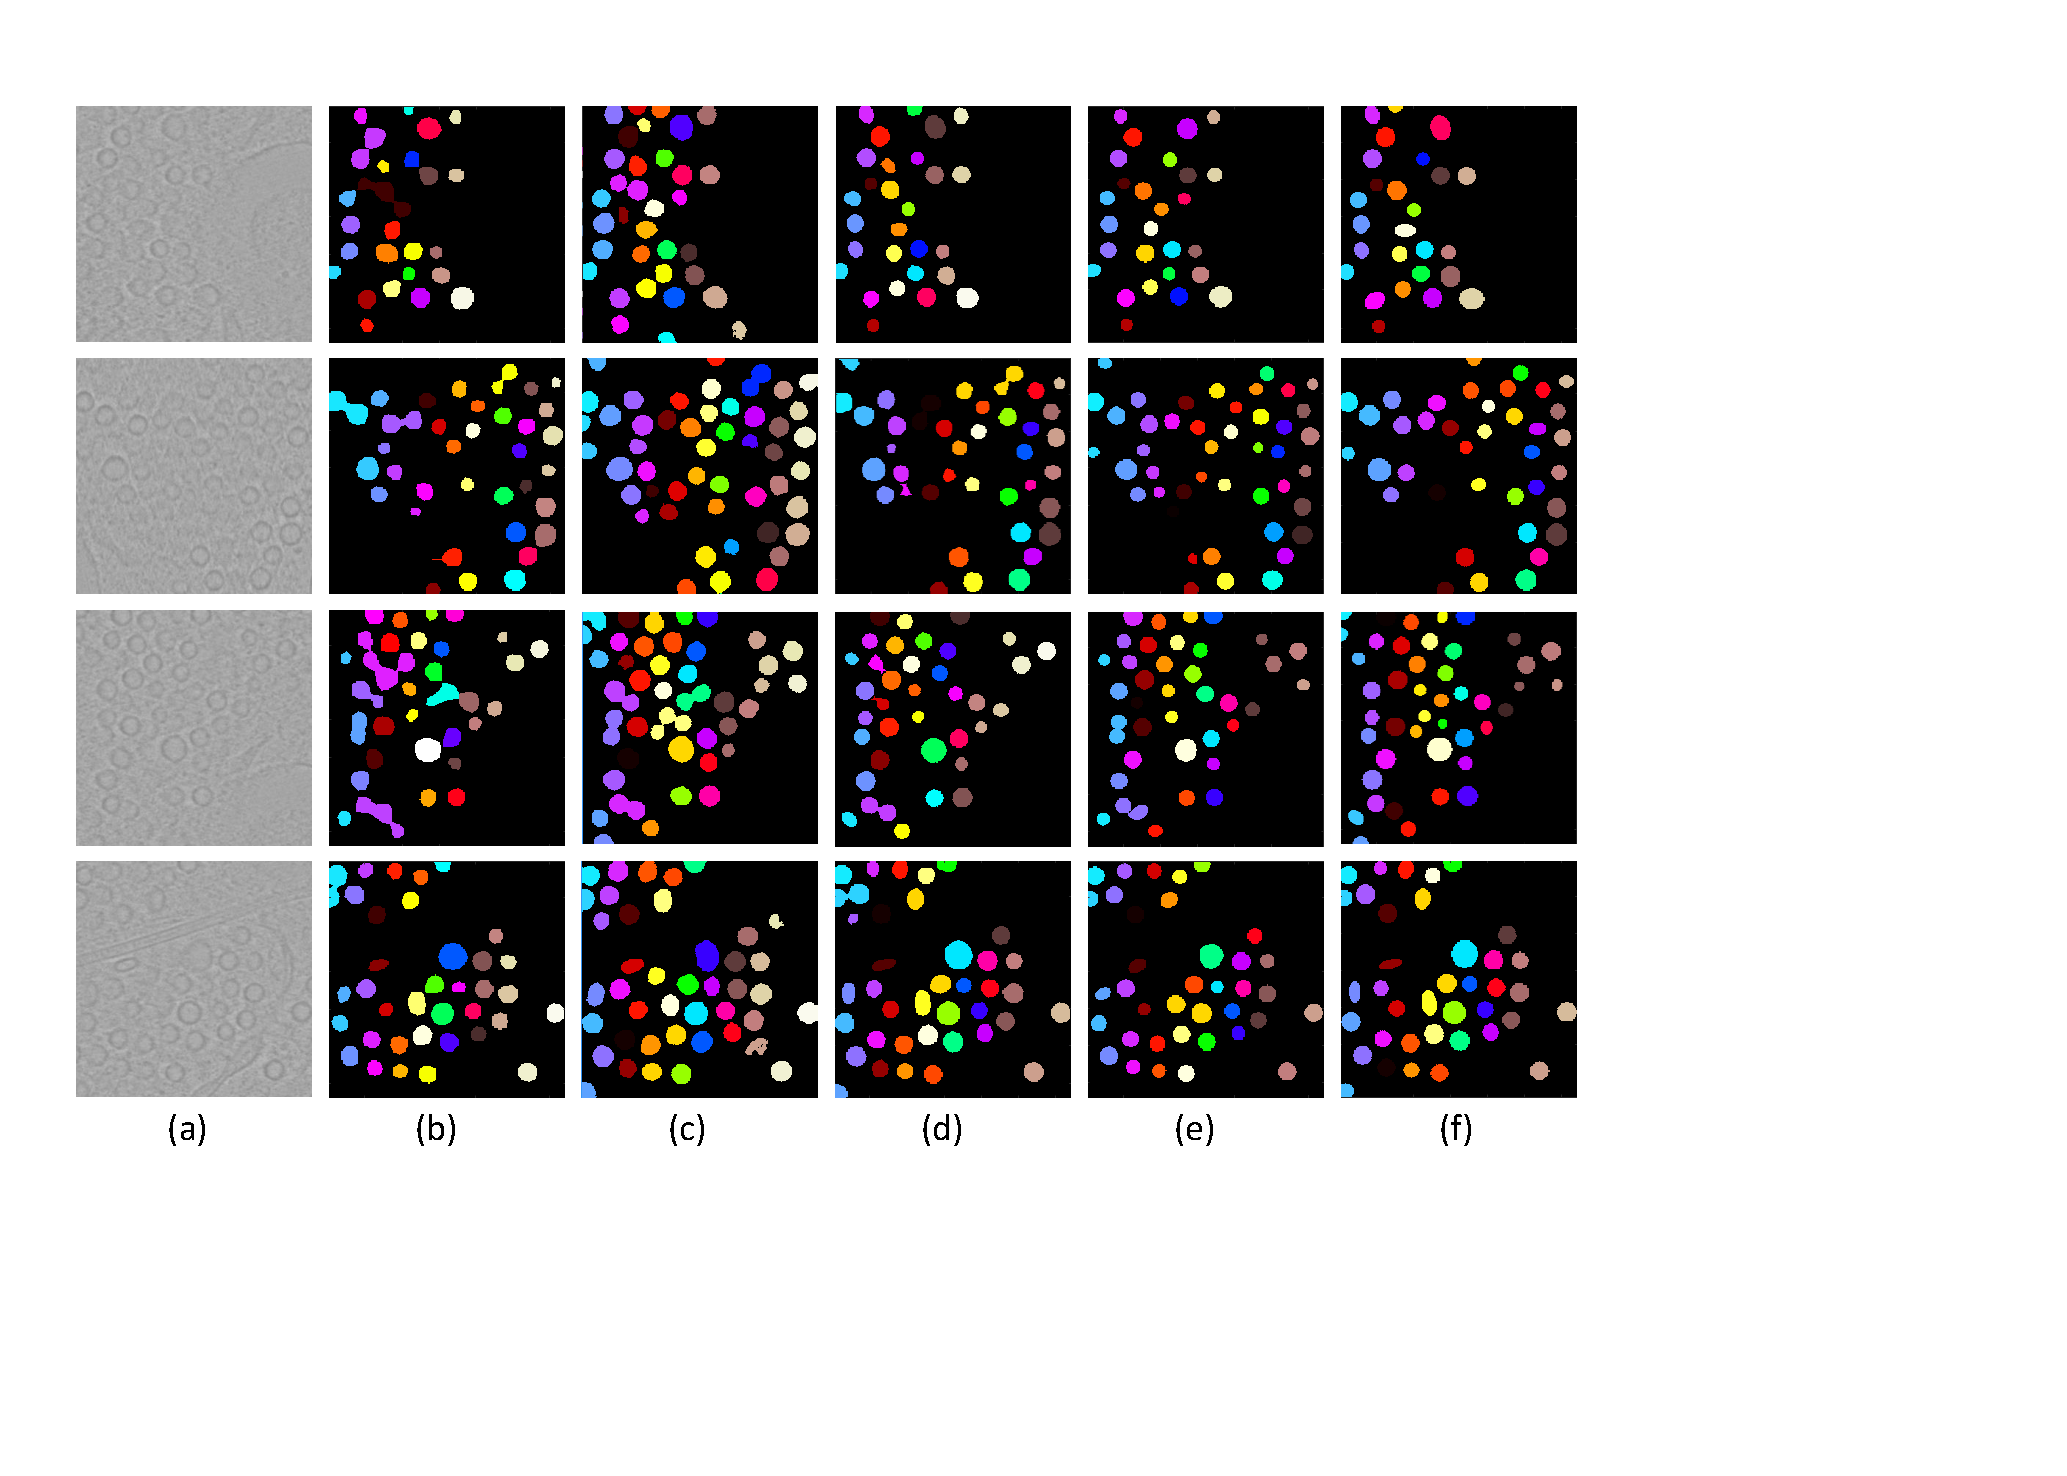
\includegraphics[width=6.8in]{figures/FigVesicle.pdf}
    \end{center}
    \caption{Some segmentation results (better seen in color) of synaptic vesicle: (a) the input image; (b)-(e) the segmentation respectively from deeplab, u-net, DCAN and DSAN; (f) the ground truth.}
    \label{FigVesicle}
\end{figure*}

Based on the above experiments, we set $\tau_1=0.2$, $\tau_2=0.9$ as the threshold setting for vesicle segmentation impose a strong shape restriction.

\noindent\textbf{Qualitative evaluation on synaptic vesicle segmentation}
Figure \ref{FigVesicle} shows some segmentation results of testing data.
In order to verify the effectiveness of parameterized shape information, we compare our method with DeepLab~\cite{Chen2014a}, u-net~\cite{Ronneberger2015} without any complementary information and DCAN~\cite{Chen2016a} with contour map as auxiliary.
The fusing thresholds follow the optimal setting in previous experiment.

\begin{table}
\begin{center}
\begin{tabular}{lcc}
\hline
Method & F1($\%$) & IOU($\%$) \\
\hline
DeepLab & 66.75 & 79.44 \\
U-net & 69.99 & 78.56 \\
DCAN & 73.94 & 81.12 \\
DSAN- & 72.52 & 80.04 \\
DSAN & $\mathbf{76.68}$ & $\mathbf{83.34}$\\
\hline
\end{tabular}
\end{center}
\caption{The detection and segmentation results of different methods in our synaptic vesicle dataset.}
\label{tab:vesicle}
\end{table}


\begin{table}
\begin{center}
\begin{tabular}{l|cccccc}
\hline
($K$,$k_s$) &deeplab& DSAN- & (1,9)& (2,4) & (3,3) & (4,2) \\
\hline
GPU time &171& 201 & 203 & 202 & 201& 203 \\
\hline
\end{tabular}
\end{center}
\caption{Average inference time (ms/image) of DSAN. DSAN- is the shape-aware network without SMP optimization.}
\label{tab:time}
\end{table}
From Figure \ref{FigVesicle}, we can see that all the methods suffer from touching problem more or less in this experiment because of the blurry and dense objects contour.
Without auxiliary, u-net (Figure~\ref{FigVesicle} (c)) performs better than DeepLab in handling touching problem due to the U-shape network.
although DCAN can solve the touching problem in many tasks, the blurry boundaries in vesicle images make it harder to obtain accurate contour maps, which leads to some touching cases in Figure~\ref{FigVesicle} (d).
Especially, the predicted shape of objects by above methods are very coarse and rough.
Differently, our DSAN uses the shape parameters of objects as complementary information to separate the touching objects apart, which obtains much more smooth and clear segmentation in Figure~\ref{FigVesicle} (e).

\noindent\textbf{Quantitative evaluation.}
To quantitatively evaluate our method, we compare the object detection rate $F_1$ and the segmentation accuracy IOU of our DSAN with Deeplab~\cite{Chen2014a}, u-net~\cite{Ronneberger2015} and DCAN~\cite{Chen2016b}, which are commonly used in biomedical image processing.
And we further implement DSAN- that is no-SMP version to prove the effectiveness of SMP.
Their results are presented in Table~\ref{tab:vesicle} to prove superiority of our method.

From the detection results, the performance of DSAN surpasses the other methods.
The common low F1 scores are caused by dense and blurry objects in vesicle dataset.
Especially, we observe that the performance of u-net obtained about $3\%$ improvement over DeepLab, both of which do not use any auxiliary supervised information.
This confirms that the missing of context information is a significant causing reason of touching problem in biomedical segmentation.
DSAN- gives a lower F1 score compared to DCAN and DSAN, because of some touching cases caused by inaccurate auxiliary information predicted in boundary regions.
And our DSAN performs better than DCAN in more challenging dense segmentation task.

From IOU metrics in Table~\ref{tab:vesicle}, our DSAN gives the best performance again among various methods.
The higher IOU score of deeplab over U-net is caused by the dilated convolution layers, which can enlarge the resolution of final predictions \cite{Chen2014a}.
The segmented vesicles by our DSAN are more clear and regular.
Both qualitative and quantitative evaluations present the superiority of our DSAN in segmenting densely arranged objects with regular and small objects by incorporating the prior shape knowledge into network.

\subsection{Gland segmentation}
\begin{figure}
    \begin{center}
        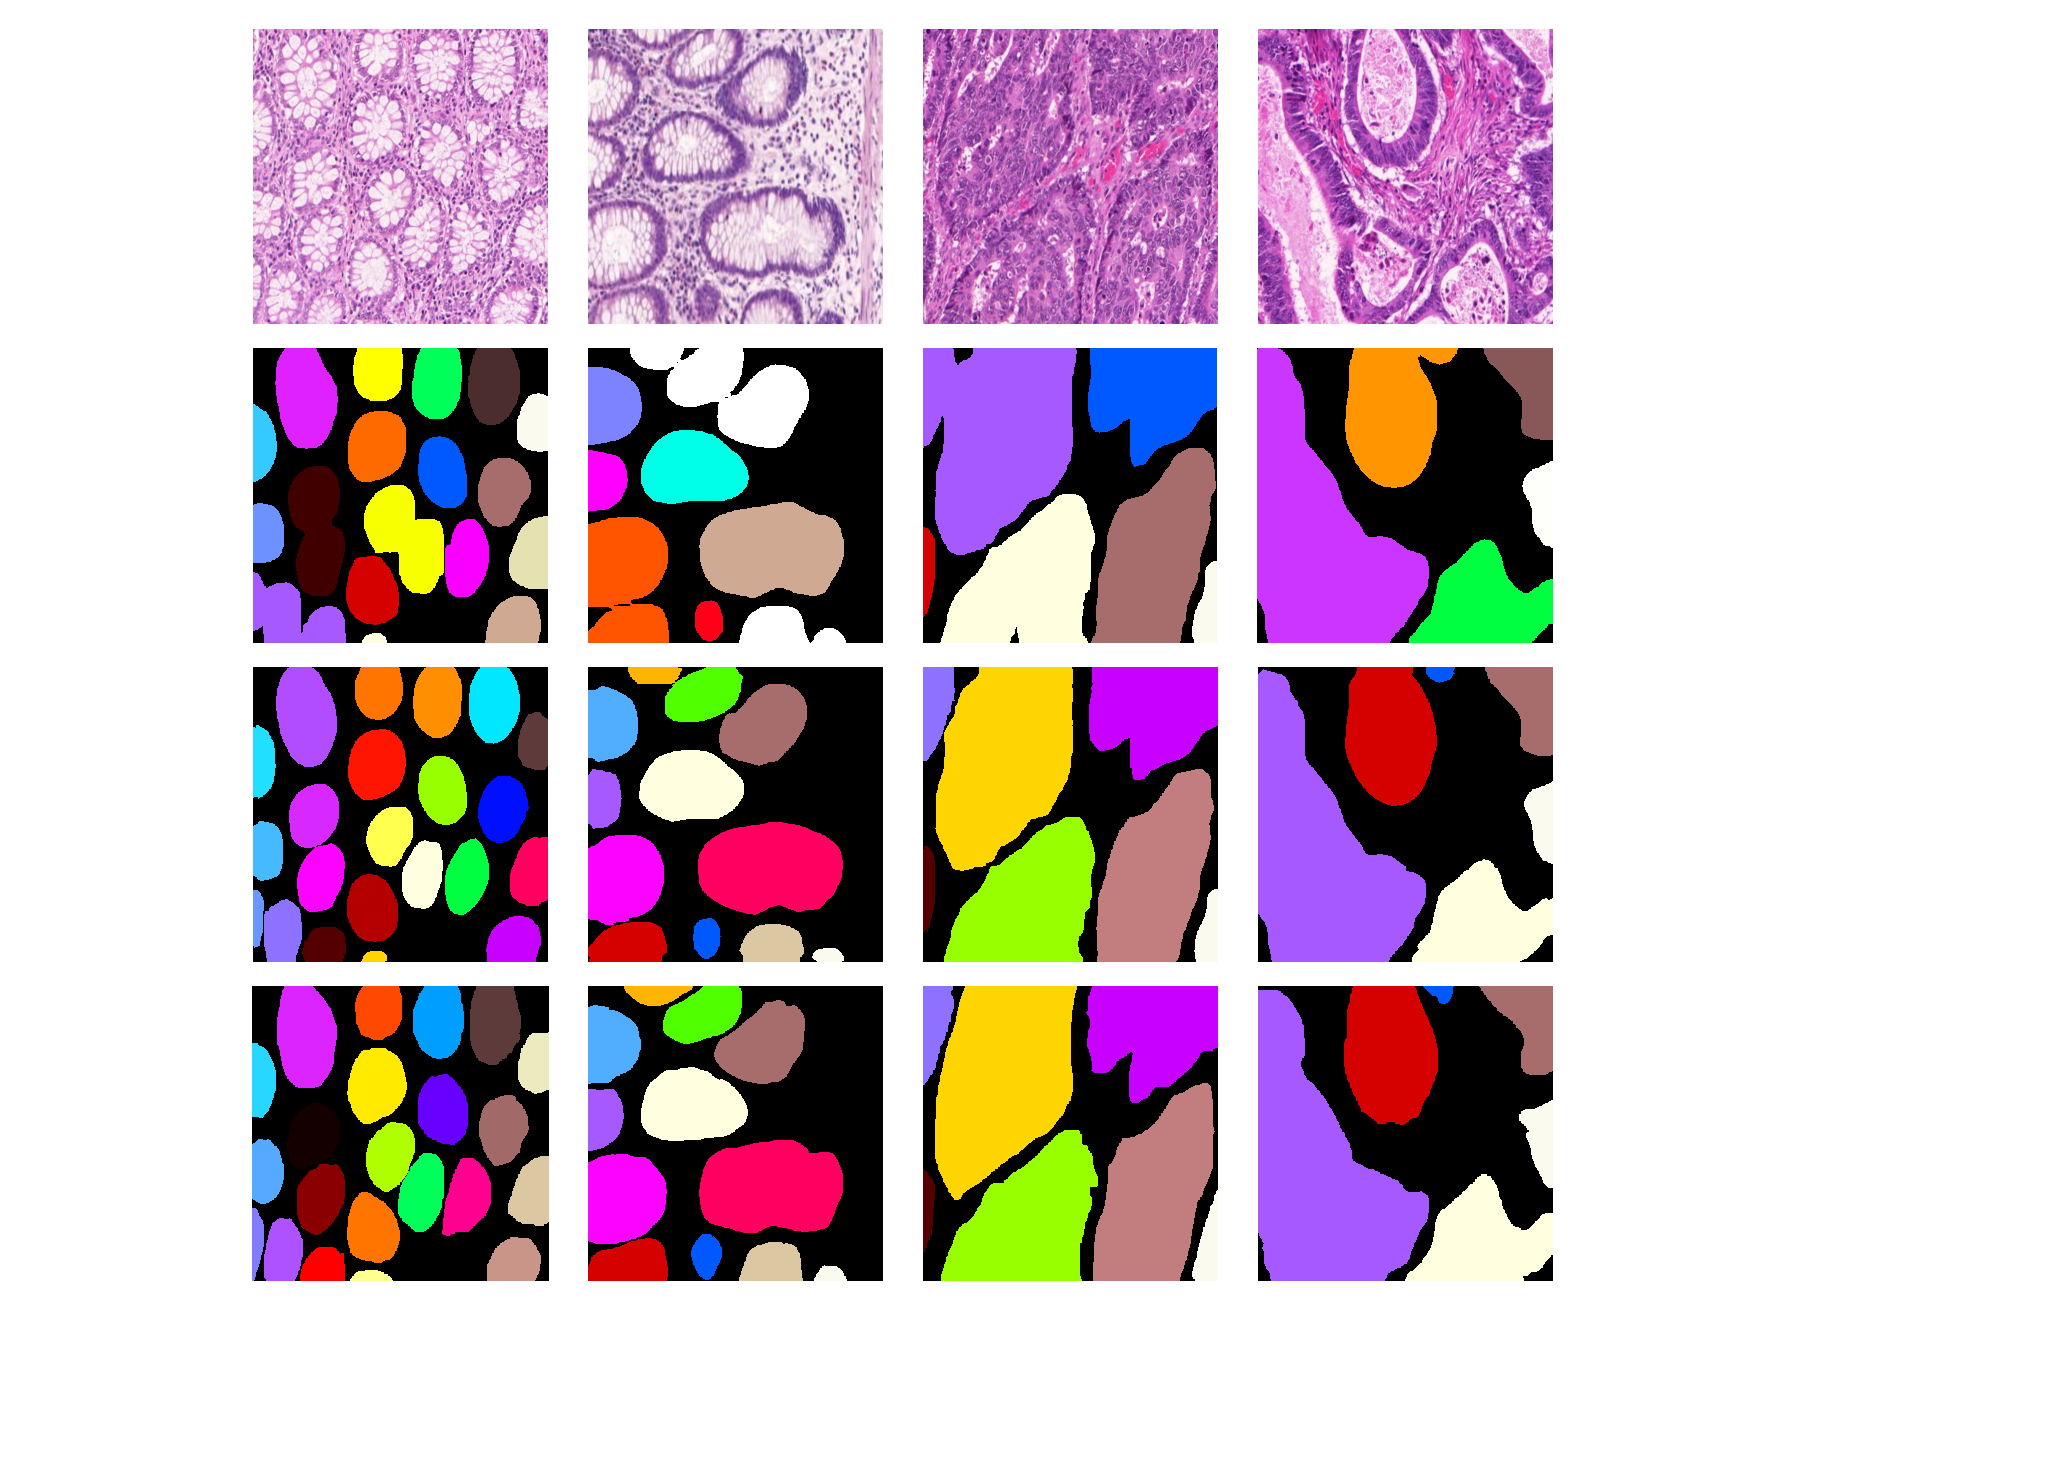
\includegraphics[width=3.3in]{figures/FigGland.pdf}
   %\includegraphics[width=0.8\linewidth]{egfigure.eps}
    \end{center}
    \caption{Several results of the gland segmentation.
    First two rows are the benign cases, and last two rows are the malignant cases.
    The results from (a) to (d) are original images, U-net, DSAN and ground truth.}
    \label{FigGland}
\end{figure}
\textbf{Dataset}
In this section we present DSAN for segmenting benign and malignant gland.
We consider the public dataset of \emph{Gland Segmentation Challenge Contest} in MICCAI2015~\cite{Sirinukunwattana2015a}.
The training dataset is composed of 85 images, consisting of 37 benign and 48 malignant, with ground truth annotations provided by expert pathologists.
The testing data contains two parts: 60 images for off-line evaluation and 20 images for on-site evaluation, and we put them together as our test dataset for evaluation.
Especially, there is a huge variation of glandular morphology in malignant case, which can prove the generalization of our DSAN to irregular objects.

\textbf{Implementation details}
Because of the large amount of irregular objects in gland images, the prior shape constraint should be weaker on predicted objects shape by objectness.
Verified by experiments, we find that $\tau_2=0.7$ and $\tau_1=0.4 $ gives the best result of our DSAN in gland segmentation.
Especially, all the images are resized to $481\times 481$ as the input to our model following \cite{Chen2014a}.
The other experiment details are similar to the settings in vesicle segmentation.

\textbf{Qualitative evaluation on gland segmentation}
For qualitative evaluation, we present the results of u-net and DSAN in Figure~\ref{FigGland} to demonstrate the effect of shape parameters in separating touching objects apart and optimizing their shapes.
The first two rows are the examples of benign gland images, and the rest two rows are the examples of malignant images.
For benign gland cases in Figure~\ref{FigGland}, we can observe an obvious advantage of auxiliary shape information in separating dense regular objects.
And for some benign cases, the predicted shape of irregular objects are also satisfied due to our piecewise fusion strategy, which retains the main shape predicted by objectness map.

\begin{table}
\begin{center}
\begin{tabular}{l|ccc}
\hline
		Method &Benign & Malignant&Overall \\
		\hline
        LIB & 80.0&47.8&62.0\\
		Freiburg2 & 91.6 & 61.6&84.9 \\
        Freihurg1 &89.3&52.1&80.4\\		
        ExB1 & 91.5 & 69.8 &86.8\\
        ExB2 & 92.0 & 68.6 &86.8\\
        ExB3 & 91.9&71.4&87.5\\
		DCAN & 91.9 & $\mathbf{77.1}$& 88.7\\
		DSAN & $\mathbf{92.2}$ & 76.8&$\mathbf{88.8}$ \\
		\hline
\end{tabular}
\end{center}
\caption{The detection results of different methods on gland segmentation dataset.}
\label{tab:gland-det}
\end{table}

\begin{table}
\begin{center}
\begin{tabular}{l|ccc}
\hline
		Method &Benign & Malignant&Overall \\
		\hline
        LIB & 81.7&66.8&74.4\\
		Freiburg2 & 90.3 & 80.1&85.3 \\
        Freihurg1 &90.3&79.8&85.2\\	
        ExB1 & 89.2 & 82.3 & 85.8\\	
        ExB2 & 90.2 & 79.9 &85.1\\
        ExB3 & 90.0&81.0&85.5\\
		DCAN & 90.7&$\mathbf{82.7}$&$\mathbf{86.8}$ \\
		DSAN & $\mathbf{91.1}$& 82.4& 86.7 \\
		\hline
\end{tabular}
\end{center}
\caption{The  segmentation results of different methods on gland segmentation dataset.}
\label{tab:gland-seg}
\end{table}

\textbf{Quantitative evaluation}
Table \ref{tab:gland-det} shows the F1 score and Table \ref{tab:gland-seg} shows object-level Dice index metric over \emph{Gland Segmentation Challenge Contest} by several published gland segmentation methods.
From the results, it can be seen that, with auxiliary shape parameters, the detection performance of our DSAN is slightly better than the results of DCAN, while the segmentation performance of DSAN is comparable.
But it should be noted that both detection and segmentation of Benign cases of our DSAN are superior than all the other methods.
And the overall performance of DSCN is still conspicuous due to its superiority in separating touching objects apart and optimizing the boundaries of regular objects, while still accommodating seriously deformable objects.
